 
\chapter{Leverage Scores and Leave-One-Out Formulas}\label{chapter::leave-one-out}
 
\section{Leverage scores}

We have seen the use of the hat matrix  $H=X(X^{\T}X)^{-1}X^{\T} $ in previous chapters. Because 
$$
H 
 = \begin{pmatrix}
x_1^{\T} \\
\vdots \\
x_{n}^{\T}
\end{pmatrix} 
(X^{\T}X)^{-1} 
\begin{pmatrix}
x_1& \cdots & x_n
\end{pmatrix},
$$
its $(i,j)$th element equals $h_{ij}=x_{i}^{\T}(X^{\T}X)^{-1}x_{j}  .$
In this chapter, we will pay special attention
to its diagonal elements 
\[
h_{ii}=x_{i}^{\T}(X^{\T}X)^{-1}x_{i}  \quad (i= 1, \ldots, n)
\]
 often called the {\it leverage scores}, which play important roles in many
discussions later. 

First, because $H$ is a projection matrix of rank $p$, we have
\[
\sumn h_{ii}=\text{trace}(H)=\text{rank}(H)=p
\]
which implies that
\[
n^{-1}\sumn h_{ii}=p/n, 
\]
i.e., the average of the leverage scores equals $p/n$ and the maximum of the leverage scores must be larger than or equal to $p/n$, which is close
to zero when $p$ is small relative to $n$. 

Second, because $H=H^{2}$ and $H=H^{\T}$, we have
$$
h_{ii}=\sum_{j=1}^{n}h_{ij}h_{ji}=\sum_{j=1}^{n}h_{ij}^{2}=h_{ii}^{2}+\sum_{j\neq i}h_{ij}^{2}\geq h_{ii}^2 
$$
which implies 
$$
h_{ii}\in[0,1] , 
$$ 
i.e., each leverage score is bounded between zero and one\footnote{This also follows from Theorem \ref{theorem::rayleigh} since the eigenvalues of $H$ are $0$ and $1$.}. 

Third, because $\hat{Y}=HY$, we have
\[
\hat{y}_{i}=\sum_{j=1}^{n}h_{ij}y_{j}=h_{ii}y_{i}+\sum_{j\neq i}h_{ij}y_{j}\]
which implies that
\[
\frac{\text{\ensuremath{\partial\hat{y}_{i}}}}{\partial y_{i}}=h_{ii}.
\]
So $h_{ii}$ measures the contribution of $y_{i}$ in the predicted
value $\hat{y}_{i}.$ In general, we do not want the contribution
of $y_{i}$ in predicting itself to be too large, because this means
we do not borrow enough information from other observations, making
the prediction very noisy. This is also clear from the variance of the predicted value 
$\hat{y}_{i}=x_{i}^{\T}\hat{\beta}$ under the Gauss--Markov model:\footnote{We have already proved a more general result on the covariance matrix of $\hat{Y}$ in Theorem \ref{thm:GMcov}.}
\begin{eqnarray*}
\text{\var}(\hat{y}_{i}) 
&=& x_{i}^{\T}\cov(\hat{\beta})x_{i} \\
&=&\sigma^{2}x_{i}^{\T}(X^{\T}X)^{-1}x_{i} \\
&=&\sigma^{2}h_{ii}.
\end{eqnarray*}
So the variance of $\hat{y}_{i}$ increases with $h_{ii}$.

The final property of $h_{ii}$ is less obvious: it measures whether
observation $i$ is an outlier based on its covariate value, that
is, whether $x_{i}$ is far from the center of the data. Partition the
design matrix as $X=\left(\begin{array}{cc}
1_{n} & X_{2}\end{array}\right)$ with $H_{1}=n^{-1}1_{n}1_{n}^{\T}.$ The covariates $X_{2}$ has sample mean $\bar{x}_{2}=n^{-1}\sumn x_{i2}$ and sample covariance 
\begin{eqnarray*}
S  
&=&  (n-1)^{-1}\sumn(x_{i2}-\bar{x}_{2})(x_{i2}-\bar{x}_{2})^{\T} \\
&=& (n-1)^{-1}X_{2}^{\T}(I_{n}-H_{1})X_{2}.
\end{eqnarray*}
The sample Mahalanobis distance between $x_{i2}$ and the center $\bar{x}_{2}$
is 
\[
D_{i}^{2}=(x_{i2}-\bar{x}_{2})^{\T}S^{-1}(x_{i2}-\bar{x}_{2}).
\]
The following theorem shows that $h_{ii}$ is a monotone function
of $D_{i}^{2}$:

\begin{theorem}\label{thm::leverage-mdist}
We have 
\begin{equation}
 h_{ii}= \frac{1}{n} + \frac{D_{i}^{2}}{n-1}  ,\label{eq:leveragemdis}
\end{equation}
so $h_{ii} \geq 1/n$. 
\end{theorem}


\begin{myproof}{Theorem}{\ref{thm::leverage-mdist}}
The definition of $D_{i}^{2}$ implies that it is the $(i,i)$th element
of the following matrix:
\begin{align*}
 & \left(\begin{array}{c}
x_{12}-\bar{x}_{2}\\
\vdots\\
x_{n2}-\bar{x}_{2}
\end{array}\right)^{\T}S^{-1}\left(\begin{array}{ccc}
x_{12}-\bar{x}_{2} & \cdots & x_{n2}-\bar{x}_{2}\end{array}\right)\\
= & (I_{n}-H_{1})X_{2}\left\{ (n-1)^{-1}X_{2}^{\T}(I_{n}-H_{1})X_{2}\right\} ^{-1}X_{2}^{\T}(I_{n}-H_{1})\\
= &(n-1)\tilde{X}_{2}(\tilde{X}_{2}^{\T}\tilde{X}_{2})^{-1}\tilde{X}_{2}^{\T}\\
= &(n-1)\tilde{H}_{2}\\
= &(n-1)(H-H_{1}),
\end{align*}
recalling that $\tilde{X}_2 = (I_n - H_1) X_2$, $\tilde{H}_2 = \tilde{X}_2 (\tilde{X}_2^{\T} \tilde{X}_2)^{-1} \tilde{X}_2^{\T}$, and $H = H_1 + \tilde{H}_{2}$ by Lemma \ref{lemma::decompose-projection-matrices}. 
Therefore, 
\[
D_{i}^{2}=(n-1) (h_{ii}-1/n)
\]
which implies (\ref{eq:leveragemdis}).
\end{myproof}




These are the basic properties of the leverage scores. 
\citet{chatterjee1988sensitivity} provided an in-depth discussion of the properties of the leverage scores. 
We will see their roles frequently in later parts of the chapter.


Another advanced result on the leverage scores is due to 
\citet{huber1973robust}. He proved that in the linear model with non-Normal IID $\varepsilon_i \sim [0, \sigma^2 ]$ and $\sigma^2 < \infty$, all linear combinations of the OLS coefficient are asymptotically Normal if and only if the maximum leverage score converges to $0$. This is a very elegant asymptotic result on the OLS coefficient. I give more details in Chapter \ref{chapter::limiting-theorems} as an application of the Lindeberg--Feller CLT.  


 

\section{Leave-one-out formulas}

To measure the impact of the $i$th observation on the final OLS estimator,
a natural approach is to delete the $i$th row from the full data

\[
X=\left(\begin{array}{c}
x_{1}^{\T}\\
\vdots\\
x_{n}^{\T}
\end{array}\right),\quad Y=\left(\begin{array}{c}
y_{1}\\
\vdots\\
y_{n}
\end{array}\right),
\]
and check how much the OLS estimator changes. Let 
$$
X_{[-i]} = \left(\begin{array}{c}
x_{1}^{\T}\\
\vdots\\
x_{i-1}^{\T} \\
x_{i+1}^{\T} \\
\vdots\\
x_{n}^{\T}
\end{array}\right),\quad 
Y_{[-i]} = \left(\begin{array}{c}
y_{1}\\
\vdots\\
y_{i-1} \\
y_{i+1} \\
\vdots\\
y_{n}
\end{array}\right)
$$ 
denote the leave-$i$-out data, and define
\begin{equation}
\hat{\beta}_{[-i]}=(X_{[-i]}^{\T}X_{[-i]})^{-1}X_{[-i]}^{\T}Y_{[-i]}\label{eq:delete1ols}
\end{equation}
as the corresponding OLS estimator. We can fit $n$ OLS by deleting
the $i$th row $(i=1,\ldots,n)$. However, this is computationally
intensive especially when $n$ is large. The following theorem shows
that we need only to fit OLS once.


\begin{theorem}\label{thm::leave-one-out-beta}
Recalling that $\hat{\beta}$ is the full data OLS, $\hat{\varepsilon}_{i}$
is the residual and $h_{ii}$ is the leverage score for the $i$th
observation, we have
\[
\hat{\beta}_{[-i]}=\hat{\beta}-(1-h_{ii})^{-1}(X^{\T}X)^{-1}x_{i}\hat{\varepsilon}_{i}
\]
if $h_{ii} \neq 1$. 
\end{theorem}
%


\begin{myproof}{Theorem}{\ref{thm::leave-one-out-beta}}
From (\ref{eq:delete1ols}), we need to invert 
\[
X_{[-i]}^{\T}X_{[-i]}=\sum_{i'\neq i}x_{i'}x_{i'}^{\T}=X^{\T}X-x_{i}x_{i}^{\T}
\]
 and calculate 
\[
X_{[-i]}^{\T}Y_{[-i]}=\sum_{i'\neq i}x_{i}y_{i}=X^{\T}Y-x_{i}y_{i},
\]
which are the original $X^{\T}X$ and $X^{\T}Y$ without the contribution of the $i$th observation. 
Using the following Sherman--Morrison formula in Problem \ref{hwmath1::inverse-block-matrix}:
\[
(A+uv^{\T})^{-1}=A^{-1}-(1+v^{\T}A^{-1}u)^{-1}A^{-1}uv^{\T}A^{-1}
\]
with $A=X^{\T}X,u=x_i$, and $v=-x_{i}$ we can invert $X_{[-i]}^{\T}X_{[-i]}$
as
\begin{align*}
(X_{[-i]}^{\T}X_{[-i]})^{-1} & =(X^{\T}X)^{-1}+\left\{ 1-x_{i}^{\T}(X^{\T}X)^{-1}x_{i}\right\} ^{-1}(X^{\T}X)^{-1}x_{i}x_{i}^{\T}(X^{\T}X)^{-1}\\
 & =(X^{\T}X)^{-1}+\left(1-h_{ii}\right)^{-1}(X^{\T}X)^{-1}x_{i}x_{i}^{\T}(X^{\T}X)^{-1}.
\end{align*}
Therefore, 
\begin{align*}
\hat{\beta}_{[-i]} & =(X_{[-i]}^{\T}X_{[-i]})^{-1}X_{[-i]}^{\T}Y_{[-i]}\\
 & =\left\{ (X^{\T}X)^{-1}+\left(1-h_{ii}\right)^{-1}(X^{\T}X)^{-1}x_{i}x_{i}^{\T}(X^{\T}X)^{-1}\right\} \left(X^{\T}Y-x_{i}y_{i}\right)\\
 & =(X^{\T}X)^{-1}X^{\T}Y \\
 &\  -(X^{\T}X)^{-1}x_{i}y_{i}\\
 & \ +\left(1-h_{ii}\right)^{-1}(X^{\T}X)^{-1}x_{i}x_{i}^{\T}(X^{\T}X)^{-1}X^{\T}Y \\
 &\ -\left(1-h_{ii}\right)^{-1}(X^{\T}X)^{-1}x_{i}x_{i}^{\T}(X^{\T}X)^{-1}x_{i}y_{i}\\
 & =\hat{\beta}-(X^{\T}X)^{-1}x_{i}y_{i}+\left(1-h_{ii}\right)^{-1}(X^{\T}X)^{-1}x_{i}x_{i}^{\T}\hat{\beta}-h_{ii}\left(1-h_{ii}\right)^{-1}(X^{\T}X)^{-1}x_{i}y_{i}\\
 & =\hat{\beta}-\left(1-h_{ii}\right)^{-1}(X^{\T}X)^{-1}x_{i}y_{i}+\left(1-h_{ii}\right)^{-1}(X^{\T}X)^{-1}x_{i}\hat{y}_{i}\\
 & =\hat{\beta}-\left(1-h_{ii}\right)^{-1}(X^{\T}X)^{-1}x_{i}\hat{\varepsilon}_{i}.
\end{align*}
\end{myproof}



With the leave-$i$-out OLS estimator $\hat{\beta}_{[-i]}$, we can
define the predicted residual
\[
\hat{\varepsilon}_{[-i]}=y_{i}-x_{i}^{\T}\hat{\beta}_{[-i]},
\]
which is different from the original residual $\hat{\varepsilon}_{i}.$ The
predicted residual based on leave-one-out can better measure the performance
of the prediction because it mimics the real problem of predicting a 
future observation. In contrast, the original residual based on the full
data $\hat{\varepsilon}_i = y_i - x_i^{\T} \hat{\beta}$ gives an overly optimistic measure of the performance of the prediction. This is related
to the overfitting issue discussed later. Under the Gauss--Markov
model, Theorem \ref{thm:GMcov} implies that the original residual
has mean zero and variance
\begin{equation}
\var(\hat{\varepsilon}_{i})=\sigma^{2}(1-h_{ii}),\label{eq:varresidualGMmodel}
\end{equation}
and we can show that the predicted residual has mean zero and variance
\begin{equation}
\var(\hat{\varepsilon}_{[-i]})=\var(y_{i}-x_{i}^{\T}\hat{\beta}_{[-i]})=\sigma^{2}+\sigma^{2}x_{i}^{\T}(X_{[-i]}^{\T}X_{[-i]})^{-1}x_{i}.\label{eq:varpresidual-1}
\end{equation}
The following theorem further simplifies the predicted residual and
its variance.

\begin{theorem}
\label{theorem:looresidual}We have 
$$
\hat{\varepsilon}_{[-i]}=\hat{\varepsilon}_{i}/(1-h_{ii}),
$$
and under Assumption \ref{assume::gm-model}, we have 
\begin{equation}
\var(\hat{\varepsilon}_{[-i]})=\sigma^{2}/(1-h_{ii}).\label{eq:varpresidual-2}
\end{equation}
\end{theorem}

\begin{myproof}{Theorem}{\ref{theorem:looresidual}}
By definition and Theorem \ref{thm::leave-one-out-beta}, we have
\begin{align}
\hat{\varepsilon}_{[-i]} & =y_{i}-x_{i}^{\T}\hat{\beta}_{[-i]}\nonumber \\
 & =y_{i}-x_{i}^{\T}\left\{ \hat{\beta}-\left(1-h_{ii}\right)^{-1}(X^{\T}X)^{-1}x_{i}\hat{\varepsilon}_{i}\right\} \nonumber \\
 & =y_{i}-x_{i}^{\T}\hat{\beta}+\left(1-h_{ii}\right)^{-1}x_{i}^{\T}(X^{\T}X)^{-1}x_{i}\hat{\varepsilon}_{i}\nonumber \\
 & =\hat{\varepsilon}_{i}+h_{ii}\left(1-h_{ii}\right)^{-1}\hat{\varepsilon}_{i}\nonumber \\
 & =\hat{\varepsilon}_{i}/(1-h_{ii})\text{.}\label{eq:predresidualformula}
\end{align}
Combining (\ref{eq:varresidualGMmodel}) and (\ref{eq:predresidualformula}), we can derive its variance formula. 
\end{myproof}


Comparing formulas (\ref{eq:varpresidual-1}) and (\ref{eq:varpresidual-2}),
we obtain that 
\[
1+x_{i}^{\T}(X_{[-i]}^{\T}X_{[-i]})^{-1}x_{i}=(1-h_{ii})^{-1}=\left\{ 1 -  x_{i}^{\T}(X^{\T}X)^{-1}x_{i}\right\} ^{-1}.
\]
This  is not an obvious linear algebra identity, but it follows immediately from
the two ways of calculating the variance of the predicted residual. 


\section{Applications of the leave-one-out formulas}

\subsection{Gauss updating formula}

Consider an online setting in which the data points come sequentially
as illustrated by the figure below:

\begin{figure}[h]
\centering
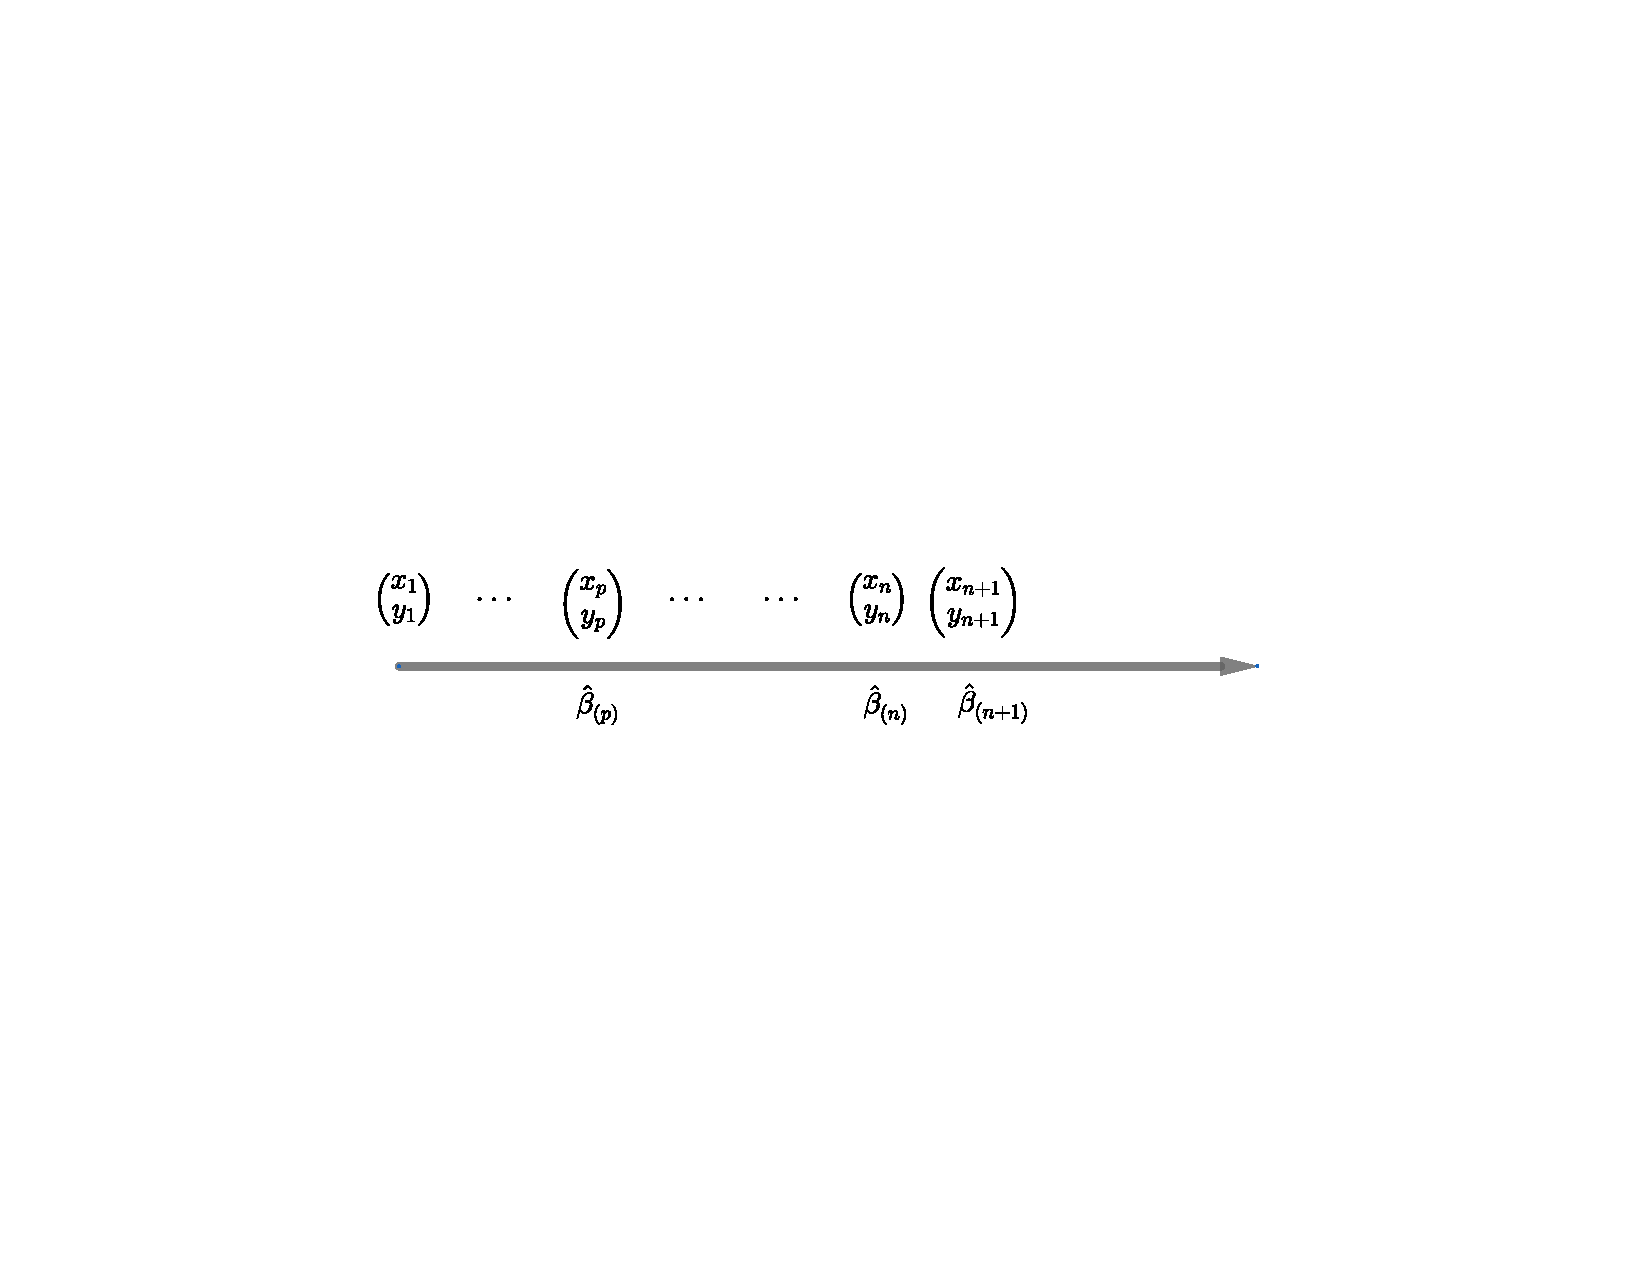
\includegraphics[width = \textwidth]{figures/gaussupdating.pdf}
\end{figure}


In this setting, we can update
the OLS estimator step by step: based on the first $n$ data points
$(x_{i},y_{i})_{i=1}^{n}$, we calculate the OLS estimator $\hat{\beta}_{(n)}$,
and with an additional data point $(x_{n+1},y_{n+1})$, we update
the OLS estimator as $\hat{\beta}_{(n+1)}$. These two OLS estimators
are closely related as shown in the following theorem. 

\begin{theorem}
\label{theorem:gaussupdate}Let $X_{(n)}$ be the design matrix and $Y_{(n)}$
be the outcome vector for the first $n$ observations. We have 
$$
\hat{\beta}_{(n+1)}=\hat{\beta}_{(n)}+\gamma_{(n+1)}\hat{\varepsilon}_{[n+1]},
$$
where $\gamma_{(n+1)}=(X_{(n+1)}^{\T}X_{(n+1)})^{-1}x_{n+1}$ and
$\hat{\varepsilon}_{[n+1]}=y_{n+1}-x_{n+1}^{\T}\hat{\beta}_{(n)}$
is the predicted residual of the $(n+1)$the outcome based on the
OLS of the first $n$ observations. 
\end{theorem}


\begin{myproof}{Theorem}{\ref{theorem:gaussupdate}}
This is the reverse form of the leave-one-out formula. We can view
the first $n+1$ data points as the full data, and $\hat{\beta}_{(n)}$
as the OLS estimator leaving the $(n+1)$the observation out.
Applying Theorem \ref{thm::leave-one-out-beta}, we have 
\begin{align*}
\hat{\beta}_{(n)} & =\hat{\beta}_{(n+1)}-(X_{(n+1)}^{\T}X_{(n+1)})^{-1}x_{n+1}\frac{\hat{\varepsilon}_{n+1}}{1-h_{n+1,n+1}}\\
 & =\hat{\beta}_{(n+1)}-\gamma_{(n+1)}\hat{\varepsilon}_{[n+1]},
\end{align*}
where $\hat{\varepsilon}_{n+1}$ is the $(n+1)$th residual based
on the full data OLS, and the $(n+1)$th predicted residual equals
$\hat{\varepsilon}_{[n+1]}=\hat{\varepsilon}_{n+1}/(1-h_{n+1,n+1})$
based on Theorem \ref{theorem:looresidual}.
\end{myproof}



Theorem \ref{theorem:gaussupdate} shows that to obtain $\hat{\beta}_{(n+1)}$
from $\hat{\beta}_{(n)}$, the adjustment depends on the predicted
residual $\hat{\varepsilon}_{[n+1]}$. If we have a perfect prediction
of the $(n+1)$th observation based on $\hat{\beta}_{(n)}$, then
we do not need to make any adjustment to obtain $\hat{\beta}_{(n+1)}$;
if the predicted residual is large, then we need to make a large
adjustment. 

Theorem \ref{theorem:gaussupdate} suggests an algorithm for sequentially
computing the OLS estimators. But it gives a formula that involves inverting $X_{(n+1)}^{\T}X_{(n+1)}$ at each step.
Using the Sherman--Morrison formula in Problem \ref{hwmath1::inverse-block-matrix}
for updating the inverse of $X_{(n+1)}^{\T}X_{(n+1)}$ based on the
inverse of $X_{(n)}^{\T}X_{(n)}$, we have an even simpler algorithm
below:
\begin{enumerate}
[(G1)]
\item\label{alg::gaussupdate1} Start with $V_{(n)}=(X_{(n)}^{\T}X_{(n)})^{-1}$ and $\hat{\beta}_{(n)}$.
\item Update 
\[
V_{(n+1)}=V_{(n)}-\left\{ 1+x_{n+1}^{\T}V_{(n)}x_{n+1}\right\} ^{-1}V_{(n)}x_{n+1}x_{n+1}^{\T}V_{(n)}.
\]
\item Calculate $\gamma_{(n+1)}=V_{(n+1)}x_{n+1}$ and $\hat{\varepsilon}_{[n+1]}=y_{n+1}-x_{n+1}^{\T}\hat{\beta}_{(n)}$.
\item\label{alg::gaussupdate4} Update $\hat{\beta}_{(n+1)}=\hat{\beta}_{(n)}+\gamma_{(n+1)}\hat{\varepsilon}_{[n+1]}$. 
\end{enumerate}
%



\subsection{Outlier detection based on residuals}

Under the Normal linear model $Y=X\beta+\varepsilon$ with $\varepsilon\sim\N(0,\sigma^{2}I_{n})$,
we know some basic probabilistic properties of the residual vector:
\[
E(\hat{\varepsilon})=0,\qquad\var(\hat{\varepsilon})=\sigma^{2}(I_{n}-H).
\]
At the same time, the residual vector is computable based on the data.
So it is sensible to check whether these properties of the residual
vector are plausible based on data, which in turn serves as modeling
checking for the Normal linear model. 

The first quantity is the standardized residual
\[
\text{standr}_{i}=\frac{\hat{\varepsilon}_{i}}{\sqrt{\hat{\sigma}^{2}(1-h_{ii})}}.
\]
We may hope that it has mean 0 and variance 1. However, because
of the dependence between $\hat{\varepsilon}_{i}$ and $\hat{\sigma}^{2}$, it is not easy to quantify the exact distribution
of $\text{standr}_{i}$. 

The second quantity is the studentized residual
based on the predicted residual:
\[
\text{studr}_{i}=\frac{\hat{\varepsilon}_{[-i]}}{\sqrt{\hat{\sigma}_{[-i]}^{2}/(1-h_{ii})}}=\frac{y_{i}-x_{i}^{\T}\hat{\beta}_{[-i]}}{\sqrt{\hat{\sigma}_{[-i]}^{2}/(1-h_{ii})}},
\]
where $\hat{\beta}_{[-i]}$ and $\hat{\sigma}_{[-i]}^{2}$ are the estimates of the coefficient and variance based
on the leave-$i$-out OLS. Because $(y_{i},\hat{\beta}_{[-i]},\hat{\sigma}_{[-i]}^{2})$
are mutually independent under the Normal linear model, we can show
that 
\begin{equation}
\text{studr}_{i}\sim t_{n-p-1}.\label{eq:studentized-t}
\end{equation}
Because we know the  distribution of $\text{studr}_{i}$, we can compare it to the quantiles
of the $t$ distribution. 

The third quantity is Cook's distance \citep{cook1977detection}:
\begin{align*}
\text{cook}_{i} & =(\hat{\beta}_{[-i]}-\hat{\beta})^{\T}X^{\T}X(\hat{\beta}_{[-i]}-\hat{\beta})/(p\hat{\sigma}^{2})\\
 & =(X\hat{\beta}_{[-i]}-X\hat{\beta})^{\T}(X\hat{\beta}_{[-i]}-X\hat{\beta})/(p\hat{\sigma}^{2}),
\end{align*}
 where the first form measures the change of the OLS estimator and
the second form measures the change in the predicted values based
on leaving-$i$-out. It has a slightly different motivation, but
eventually, it is related to the previous two residuals due to the leave-one-out formulas. 

\begin{theorem}\label{thm::cooksdist-standr}
Cook's distance is related to the standardized residual via:
\[
\textup{cook}_{i}=\textup{standr}_{i}^{2}\times\frac{h_{ii}}{p(1-h_{ii})}.
\]
\end{theorem}

I leave the proof of Theorem \ref{thm::cooksdist-standr}  as Problem \ref{hw10::cooks-standr}. 



I will end this subsubsection with two examples. The \ri{R} code is in \ri{code11.3.2.R}. The first one is simulated. 
I generate data from a univariate Normal linear model without outliers. I then use \ri{hatvalues}, \ri{r.standard}, \ri{r.student} and \ri{cooks.distance} to an \ri{lm.object} to calculate the leverage scores, standardized residuals, studentized residuals, and Cook's distances. Their plots are in the first column of Figure \ref{fig::outlier-detections}. 
\begin{lstlisting}
n = 100
x = seq(0, 1, length = n)
y = 1 + 3*x + rnorm(n)
lmmod = lm(y ~ x)
hatvalues(lmmod)
rstandard(lmmod)
rstudent(lmmod)
cooks.distance(lmmod)
\end{lstlisting}
If I add $8$ to the outcome of the last observation, the plots change to the second column of Figure \ref{fig::outlier-detections}. If I add $8$ to the $50$th observation, the plots change to the last column of Figure \ref{fig::outlier-detections}. Both visually show the outliers. 
 In this example, the three residual plots give qualitatively the same pattern, so the choice among them does not matter much. In general cases, we may prefer $\text{studr}_{i}$ because it has a known distribution under the Normal linear model. 

\begin{figure}[ht]
\centering
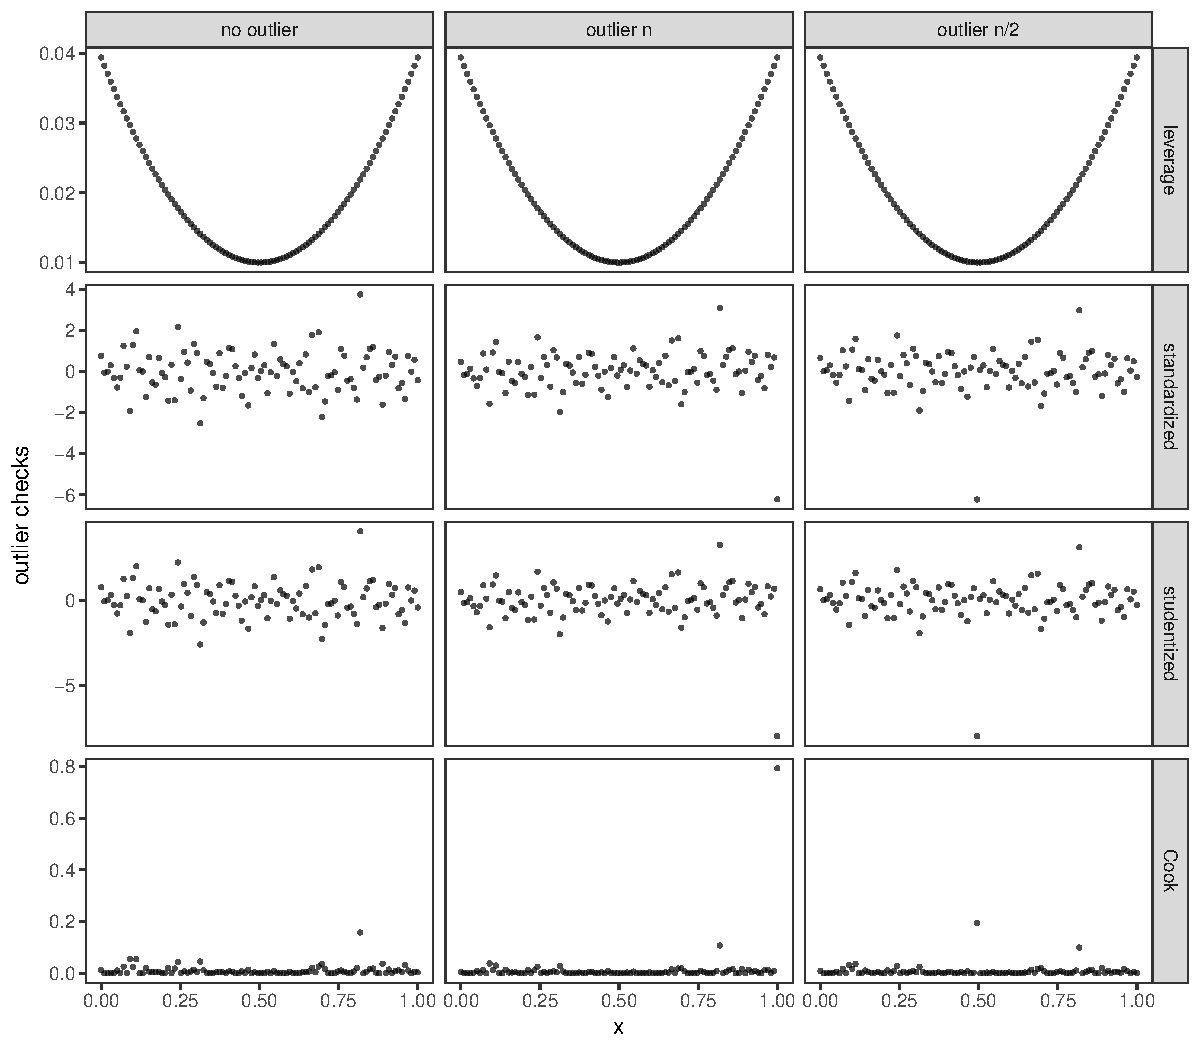
\includegraphics[width = \textwidth]{figures/residual_diagnostics.pdf}
\caption{Outlier detections}\label{fig::outlier-detections}
\end{figure}




The second one is a further analysis of the Lalonde data. Based on the plots in Figure \ref{fig::outlier-detections-lalonde}, there are indeed some outliers in the data. It is worth investigating them more carefully. 

\begin{figure}[ht]
\centering
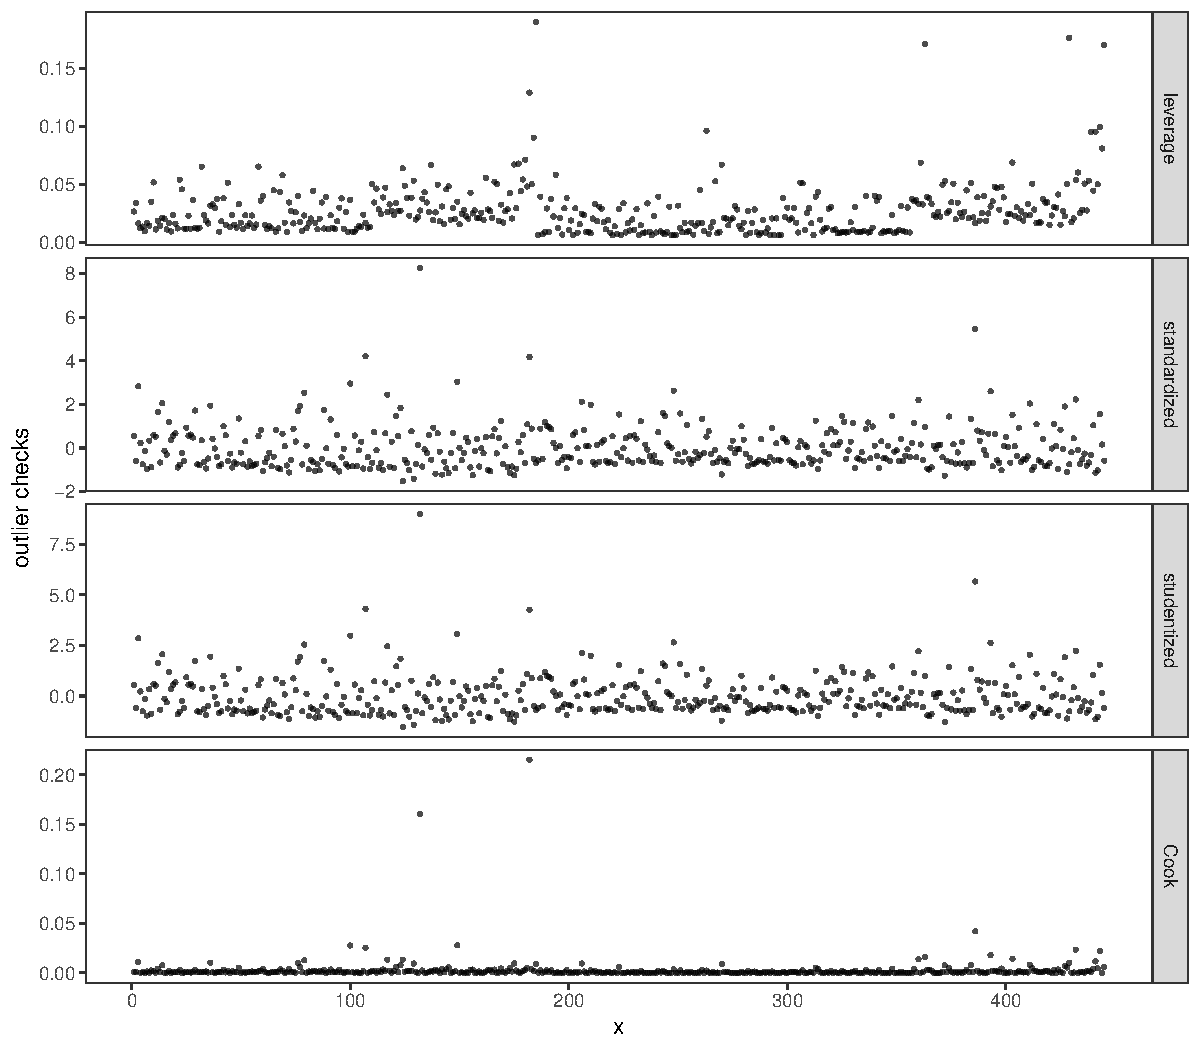
\includegraphics[width = \textwidth]{figures/residual_diagnostics_lalonde.pdf}
\caption{Outlier detections in the LaLonde data}\label{fig::outlier-detections-lalonde}
\end{figure}



Although the outliers detection methods above are very classic, they are rarely implemented in modern data analyses. They are simple and useful diagnostics. I recommend using them at least as a part of the exploratory data analysis.  

 
 
\subsection{Jackknife} 
 

Jackknife is a general strategy for bias reduction and variance estimation proposed by \citet{quenouille1949approximate, quenouille1956notes} and popularized by  \citet{tukey1958bias}. Based on independent data $(Z_1,\ldots,Z_n)$, how to estimate the variance of a general estimator $\hat{\theta}(Z_1,\ldots,Z_n)$ of the parameter $\theta$? Define $\hat{\theta}_{[-i]}$ as the estimator without observation $i$, and the pseudo-value as 
$$
\tilde{\theta}_i = n \hat{\theta} - (n-1) \hat{\theta}_{[-i]} .
$$ 
The jackknife point estimator is $\hat{\theta}_\textsc{j} = n^{-1} \sumn \tilde{\theta}_i$, and the jackknife variance estimator is 
 $$
\hat{V}_\textsc{j}  = \frac{1}{n(n-1)}\sumn (\tilde{\theta}_i  - \hat{\theta}_\textsc{j}  )(\tilde{\theta}_i - \hat{\theta}_\textsc{j}  )^{\T}.
 $$


We have already shown that the OLS coefficient is unbiased and derived several variance estimators for it. 
Here we focus on the jackknife in OLS using the leave-one-out formula for the coefficient. The pseudo-value is
\begin{eqnarray*}
\tilde{\beta}_i &=& n \hat{\beta} - (n-1) \hat{\beta}_{[-i]} \\
&=& n \hat{\beta} - (n-1) \left\{ \hat{\beta}-(1-h_{ii})^{-1}(X^{\T}X)^{-1}x_{i}\hat{\varepsilon}_{i} \right\} \\
&=& \hat{\beta}  + (n-1)  (1-h_{ii})^{-1}(X^{\T}X)^{-1}x_{i}\hat{\varepsilon}_{i} .
\end{eqnarray*}
The jackknife point estimator is 
$$
\hat{\beta}_\textsc{j} = \hat{\beta} + \frac{n-1}{n} \left( n^{-1} \sumn x_i x_i^{\T} \right)^{-1} 
\left(   n^{-1} \sumn x_{i}  \frac{  \hat{\varepsilon}_{i} }{ 1-h_{ii} }   \right) .
$$
 It is a little unfortunate that the jackknife point estimator is not identical to the OLS estimator, which is BLUE under the Gauss--Markov model.  
We can show that  $E(\hat{\beta}_\textsc{j} )  = \beta$ and it is a linear estimator. So the Gauss--Markov theorem ensures that $\cov( \hat{\beta}_\textsc{j} ) \succeq \cov( \hat{\beta})$. 
 
 
 Nevertheless, the difference between $\hat{\beta}_\textsc{j}$ and $\hat{\beta}$  is quite small. I omit their difference in the following derivation. Assuming that $\hat{\beta}_\textsc{j}  \cong \hat{\beta} $, we can continue to calculate the approximate jackknife variance estimator:
\begin{eqnarray*}
\hat{V}_\textsc{j} &\cong& \frac{1}{n(n-1)} \sumn (\tilde{\beta}_i - \hat{\beta})(\tilde{\beta}_i  - \hat{\beta})^{\T} \\
&=& \frac{n-1}{n} (X^{\T}X)^{-1}  \sumn \left(  \frac{  \hat{\varepsilon}_{i}  }{ 1-h_{ii}} \right)^2 x_{i}x_{i}^{\T}  (X^{\T}X)^{-1},
\end{eqnarray*} 
which is almost identical to the HC3 form of the EHW covariance matrix introduced in Chapter \ref{sec::HCs}. \citet{miller1974unbalanced} first analyzed the jackknife in OLS but dismissed it immediately. \citet{hinkley1977jackknifing} modified the original jackknife and proposed a version that is identical to HC1, and \citet{wu1986jackknife} proposed some further modifications and proposed a version that is identical to HC2. 
\citet{weber1986jackknife} made connections between EHW and jackknife standard errors. 
However, \citet{long2000using}'s finite-sample simulation seems to favor the original jackknife or HC3. 




\section{Homework problems}





\paragraph{Implementing the Gauss updating formula}
Implement the algorithm in (G\ref{alg::gaussupdate1})--(G\ref{alg::gaussupdate4}), and try it on simulated data. 


\paragraph{The distribution of the studentized residual}

Prove (\ref{eq:studentized-t}).

\paragraph{Leave-one-out coefficient}\label{hw10::loo-coefficient}

Prove 
\[
\hat{\beta}=\sumn w_{i}\hat{\beta}_{[-i]},
\]
and find the weights $w_{i}$'s. Show they are positive and sum to
one. Does $\hat{\beta}=n^{-1}\sumn\hat{\beta}_{[-i]}$ hold in general?

\paragraph{Cook's distance and the standardized residual}\label{hw10::cooks-standr}

Prove Theorem \ref{thm::cooksdist-standr}. 


\paragraph{The relationship between the standardized and studentized residual}\label{hw10::residuals-relationship}

Prove the following results. 
\begin{enumerate}
\item $(n-p-1)\hat{\sigma}_{[-i]}^{2}=(n-p)\hat{\sigma}^{2}-\hat{\varepsilon}_{i}^{2}/(1-h_{ii})$. 

 


\item There is a monotone relationship between the standardized and studentized
residual:
\[
\text{studr}_{i}=\text{standr}_{i}\sqrt{\frac{n-p-1}{n-p-\text{standr}_{i}^{2}}}.
\]
\end{enumerate}

Remark: The right-hand side of the first result must be nonnegative so  $\sum_{k=1}^n   \hat{\varepsilon}_k^2 \geq \hat{\varepsilon}_{i}^{2}/(1-h_{ii})$, which 
implies the following inequality:
$$
h_{ii}  + \frac{  \hat{\varepsilon}_i^2 }{ \sum_{k=1}^n   \hat{\varepsilon}_k^2 } \leq 1.
$$
From this inequality, if $h_{ii} = 1$ then $\hat{\varepsilon}_i = 0$ which further implies that $h_{ij} = 0$ for all $j \neq i.$
 


 


%\paragraph{Exact form of the jackknife variance estimate} Without any approximations, derive the exact form of $\hat{V}_\textsc{j}$ for the OLS coefficient. 


\paragraph{Subset and full-data OLS coefficients}
\label{hw10::subset-ols-coef}


Leaving one observation out, we have the OLS coefficient formula in Theorem \ref{thm::leave-one-out-beta}. Leave a subset of observations out, we have the OLS coefficient formula below. Partition the covariate matrix and outcome vector based on a subset $S$ of $\{1, \ldots, n\}$:
$$
X = \begin{pmatrix}
X_S\\
X_{\backslash S}
\end{pmatrix},\qquad 
Y = \begin{pmatrix}
Y_S\\
Y_{\backslash S}
\end{pmatrix} .
$$  
Without using the observations in set $S$, we have the OLS coefficient 
$$
\hat\beta_{\backslash S} = (X_{\backslash S}^{\T} X_{\backslash S})^{-1} X_{\backslash S}Y_{\backslash S}.
$$
The following formula facilitates the computation of many $\hat\beta_{\backslash S} $'s simultaneously, which relies crucially on the subvector of the residuals 
$$
\hat{\varepsilon}_S = Y_S - X_S\hat\beta_{\backslash S} 
$$  
and the submatrix of $H$
$$
H_{SS} = X_{\backslash S}(X^{\T}X)^{-1}X_{\backslash S}^{\T}
$$
corresponding to the set $S$. 

\begin{theorem}\label{thm::leave-subset-out-beta}
Recalling that $\hat{\beta}$ is the full data OLS, we have
\[
\hat\beta_{\backslash S}   =\hat{\beta}- (X^{\T}X)^{-1}  X_{\backslash S}^{\T} (I-H_{SS})^{-1} \hat{\varepsilon}_S 
\]
where $I$ is the identity matrix with the same dimension of $H_{SS}$. 
\end{theorem}


Prove Theorem \ref{thm::leave-subset-out-beta}. 





\paragraph{Bounding the leverage score}
\label{hw10::bounding-h-more}


Theorem \ref{thm::leverage-mdist} shows $ n^{-1} \leq h_{ii} \leq 1$ for all $i = 1, \ldots , n$.
Prove the following stronger result:
$$
n^{-1} \leq h_{ii} \leq   s_i^{-1}
$$
where $s_i$ is the number of rows that are identical to $x_i$ or $-x_i$.



 

\paragraph{More on the leverage score}
\label{hw10::h-grammatrix}
 
Show that 
$$
\text{det}(X_{[-i]}^{\T}X_{[-i]}) = (1-h_{ii}) \text{det}(X^{\T} X). 
$$ 
 
 
 
Remark: If $h_{ii} =1$, then $X_{[-i]}^{\T}X_{[-i]}$ is degenerate with determinant $0$. Therefore, if we delete an observation $i$ with leverage score $1$, the columns of the covariate matrix become linearly dependent. 
